\documentclass[tikz, border=10pt]{standalone}
\usepackage{tikz}
\usepackage{amsmath}
\usetikzlibrary{positioning, arrows.meta, shapes, backgrounds, fit, calc}

\usepackage{helvet}
\renewcommand{\familydefault}{\sfdefault}
\usepackage{sansmath}
\sansmath

% UCL brand accessible data-viz palette (matches marvel_algorithm.tex / marvel_breaks.tex)
\definecolor{uclDarkPurple}{HTML}{361A54}
\definecolor{uclLightPink}{HTML}{E645AB}
\definecolor{uclLightOrange}{HTML}{E66C37}
\definecolor{uclLightGreen}{HTML}{1AAB40}
\definecolor{uclLightBlue}{HTML}{118DFF}
\definecolor{uclDarkRed}{HTML}{751441}

\begin{document}

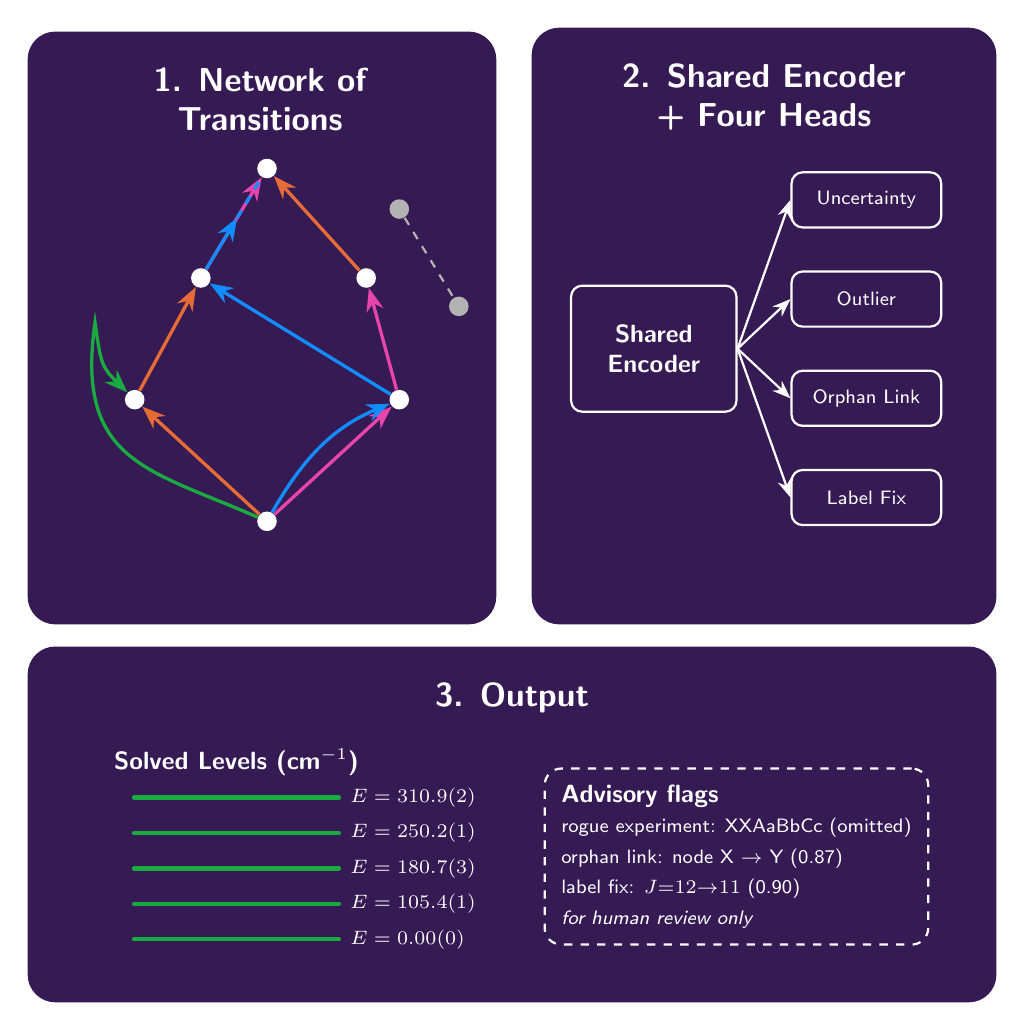
\begin{tikzpicture}[
    font=\sffamily,
    >=Stealth,
    node distance=1cm,
    every node/.style={text=white},
    level_dot/.style={circle, fill=white, inner sep=2.5pt},
    orphan_dot/.style={circle, fill=gray!60, inner sep=2.5pt},
    level_line/.style={ultra thick, uclLightGreen, line cap=round},
    srcA/.style={->, very thick, color=uclLightOrange},
    srcB/.style={->, very thick, color=uclLightPink},
    srcC/.style={->, very thick, color=uclLightBlue},
    srcC_gap/.style={-, very thick, dashed, color=uclLightBlue},
    orphan_edge/.style={-, thick, dashed, gray!60},
    flagged_edge/.style={->, very thick, color=uclLightGreen},
    head_box/.style={rectangle, rounded corners=4pt, draw=white, thick, fill=uclDarkPurple, minimum width=1.9cm, minimum height=0.7cm, align=center, font=\scriptsize},
    encoder_box/.style={rectangle, rounded corners=4pt, draw=white, thick, fill=uclDarkPurple, minimum width=2.1cm, minimum height=1.6cm, align=center, font=\bfseries\small},
    advisory_box/.style={rectangle, rounded corners=6pt, draw=white, thick, dashed, minimum width=3.6cm, align=left, font=\small, inner sep=6pt},
    panel_bg/.style={rounded corners=10pt, inner sep=10pt, draw=none},
    heading/.style={font=\bfseries\large, align=center, anchor=south}
]

% Shared geometry: two equal-width boxes on top, one box across the bottom
% at double their width (+ the gap between them), so all three edges line up.
\def\topW{5.2}
\def\topH{6.30}
\def\gapX{1.2}
\def\gapY{1.2}
\def\botW{11.6} % = 2*\topW + \gapX
\def\botH{3.6}

%% --- BOX 1 (top-left): NETWORK OF TRANSITIONS ---
%% Same jumbled network as the end state of marvel_breaks.tex (clean network +
%% orphan cluster + looping mislabel + near-miss new source), T-labels dropped
%% -- just nodes and arrows -- scaled up to fill the extra room this box gets.
\begin{scope}[local bounding box=p1]
    \path (0,0) rectangle (\topW,\topH);

    \node[heading] at (2.6, 5.80) {1. Network of\\Transitions};

    \begin{scope}[xscale=0.84, yscale=1.03, shift={(-1.20,1.68)}]
        \node[level_dot] (G) at (4.4, -0.75) {};
        \node[level_dot] (A) at (2.4, 0.75) {};
        \node[level_dot] (B) at (6.4, 0.75) {};
        \node[level_dot] (C) at (3.4, 2.25) {};
        \node[level_dot] (D) at (5.9, 2.25) {};
        \node[level_dot] (E) at (4.4, 3.6) {};
        \node[orphan_dot] (X) at (6.4, 3.1) {};
        \node[orphan_dot] (Y) at (7.3, 1.9) {};

        \draw[srcA] (G) -- (A);
        \draw[srcB] (G) -- (B);
        \draw[srcA] (A) -- (C);
        \draw[srcB] (B) -- (D);
        \draw[srcA] (D) -- (E);
        \draw[srcB] (C) -- (E);
        \draw[orphan_edge] (X) -- (Y);

        \coordinate (t7curl) at ($(A)+(-0.6,0.95)$);
        \draw[flagged_edge] (G) to[out=160, in=260, looseness=1.3] (t7curl)
            to[out=-80, in=140, looseness=1.3] (A);

        \draw[srcC] (G) to[bend left=18] (B);
        \draw[srcC] (B) -- (C);
        \draw[srcC] (C) -- ($(C)!0.55!(E)$);
        \draw[srcC_gap] ($(C)!0.55!(E)$) -- ($(C)!0.9!(E)$);
    \end{scope}
\end{scope}

%% --- BOX 2 (top-right): SHARED ENCODER -> FOUR HEADS ---
%% Same width as Box 1, so the extra height gives the encoder and its four
%% heads room to sit neatly, evenly spaced, aligned with one another.
\begin{scope}[xshift=6.4cm, local bounding box=p2]
    \path (0,0) rectangle (\topW,\topH);

    \node[heading] at (2.6, 5.80) {2. Shared Encoder\\+ Four Heads};

    \node[encoder_box] (enc) at (1.2, 3.15) {Shared\\Encoder};

    \node[head_box] (h1) at (3.9, 5.04) {Uncertainty};
    \node[head_box] (h2) at (3.9, 3.78) {Outlier};
    \node[head_box] (h3) at (3.9, 2.52) {Orphan Link};
    \node[head_box] (h4) at (3.9, 1.26) {Label Fix};

    \draw[->, white, thick] (enc.east) -- (h1.west);
    \draw[->, white, thick] (enc.east) -- (h2.west);
    \draw[->, white, thick] (enc.east) -- (h3.west);
    \draw[->, white, thick] (enc.east) -- (h4.west);
\end{scope}

%% --- BOX 3 (bottom, full width): OUTPUT ---
%% Left half: solved levels. Right half: advisory flags.
\begin{scope}[yshift=-4.8cm, local bounding box=p3]
    \path (0,0) rectangle (\botW,\botH);

    \node[heading] at (5.8, 3.2) {3. Output};

    % 3a: Solved levels (left half), with an uncertainty band
    \node[font=\bfseries\small] at (2.3, 2.7) {Solved Levels (cm$^{-1}$)};
    \draw[level_line] (1.0,2.25) -- (3.6,2.25) node[right, font=\scriptsize] {$E=310.9(2)$};
    \draw[level_line] (1.0,1.8) -- (3.6,1.8) node[right, font=\scriptsize] {$E=250.2(1)$};
    \draw[level_line] (1.0,1.35) -- (3.6,1.35) node[right, font=\scriptsize] {$E=180.7(3)$};
    \draw[level_line] (1.0,0.9) -- (3.6,0.9) node[right, font=\scriptsize] {$E=105.4(1)$};
    \draw[level_line] (1.0,0.45) -- (3.6,0.45) node[right, font=\scriptsize] {$E=0.00(0)$};

    % 3b: Advisory flags (right half) -- dashed border marks human-review-only outputs
    \node[advisory_box] (adv) at (8.65, 1.5) {
        \textbf{Advisory flags}\\
        {\scriptsize rogue experiment: XXAaBbCc (omitted)}\\
        {\scriptsize orphan link: node X $\to$ Y (0.87)}\\
        {\scriptsize label fix: $J{=}12{\to}11$ (0.90)}\\
        {\scriptsize\itshape for human review only}
    };
\end{scope}

%% --- BACKGROUND LAYERS ---
\begin{scope}[on background layer]
    \node[panel_bg, fill=uclDarkPurple, fit=(p1)] (bg1) {};
    \node[panel_bg, fill=uclDarkPurple, fit=(p2)] (bg2) {};
    \node[panel_bg, fill=uclDarkPurple, fit=(p3)] (bg3) {};
\end{scope}

\end{tikzpicture}
\end{document}
